\documentclass{beamer}
% \documentclass[handout]{beamer}
\usetheme{Warsaw}

\setbeamercolor{normal text}{fg=white,bg=black!90}
\setbeamercolor{structure}{fg=white}

\setbeamercolor{alerted text}{fg=red!85!black}

\setbeamercolor{item projected}{use=item,fg=black,bg=item.fg!35}

\setbeamercolor*{palette primary}{use=structure,fg=structure.fg}
\setbeamercolor*{palette secondary}{use=structure,fg=structure.fg!95!black}
\setbeamercolor*{palette tertiary}{use=structure,fg=structure.fg!90!black}
\setbeamercolor*{palette quaternary}{use=structure,fg=structure.fg!95!black,bg=black!80}

\setbeamercolor*{framesubtitle}{fg=white}

\setbeamercolor*{block title}{parent=structure,bg=black!60}
\setbeamercolor*{block body}{fg=black,bg=black!10}
\setbeamercolor*{block title alerted}{parent=alerted text,bg=black!15}
\setbeamercolor*{block title example}{parent=example text,bg=black!15}

\definecolor{blue}{rgb}{0,0.5,1}

\graphicspath{{figures/}}

\usepackage[ngerman]{babel}

\title{Informatik: Zahlensysteme}
% \subtitle{}
\author{sca,kng}
\institute{KSR}
\date{\today}

\begin{document}

\begin{frame}
    \titlepage
\end{frame}

\begin{frame}
    \LARGE
    Lektion 2: Dezimal- \& Binärsystem
\end{frame}

\begin{frame}
    \frametitle{Warm-Up I}
    Uhrzeit 1:
    \begin{figure}[H]
        \centering
        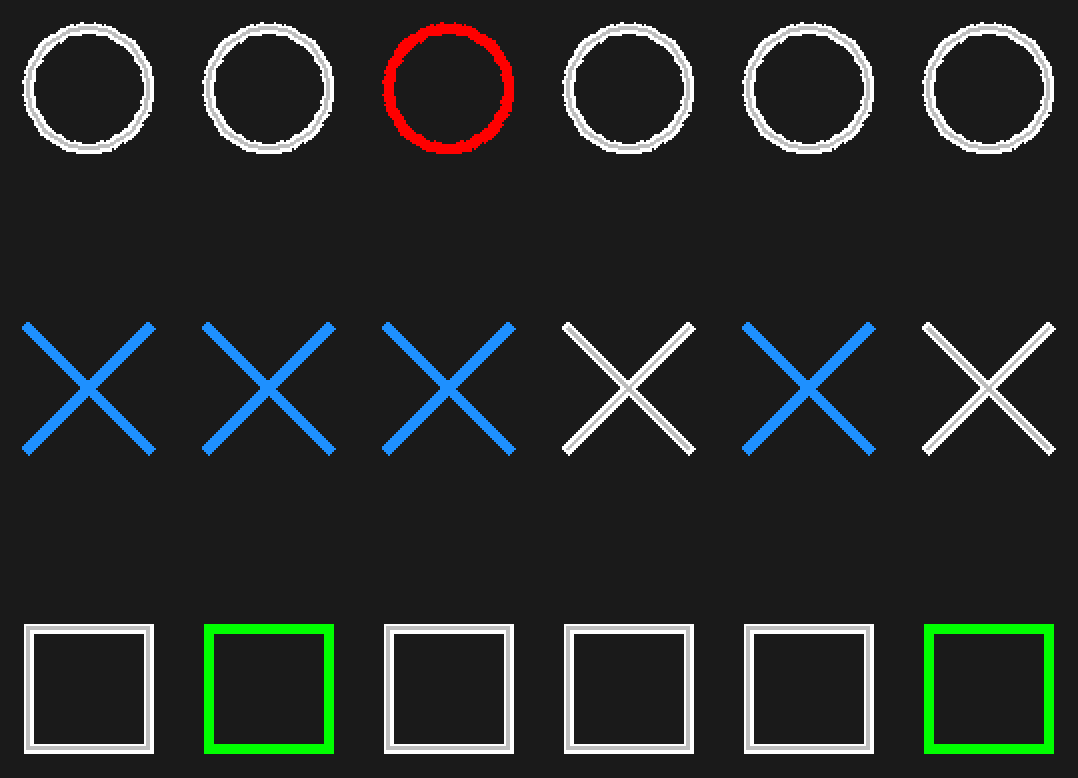
\includegraphics[width=0.7\textwidth]{08_58_17_dark}
    \end{figure}
    \onslide<2-> $$08:58:17$$
\end{frame}

\begin{frame}
    \frametitle{Warm-Up I}
    \begin{figure}[H]
        \centering
        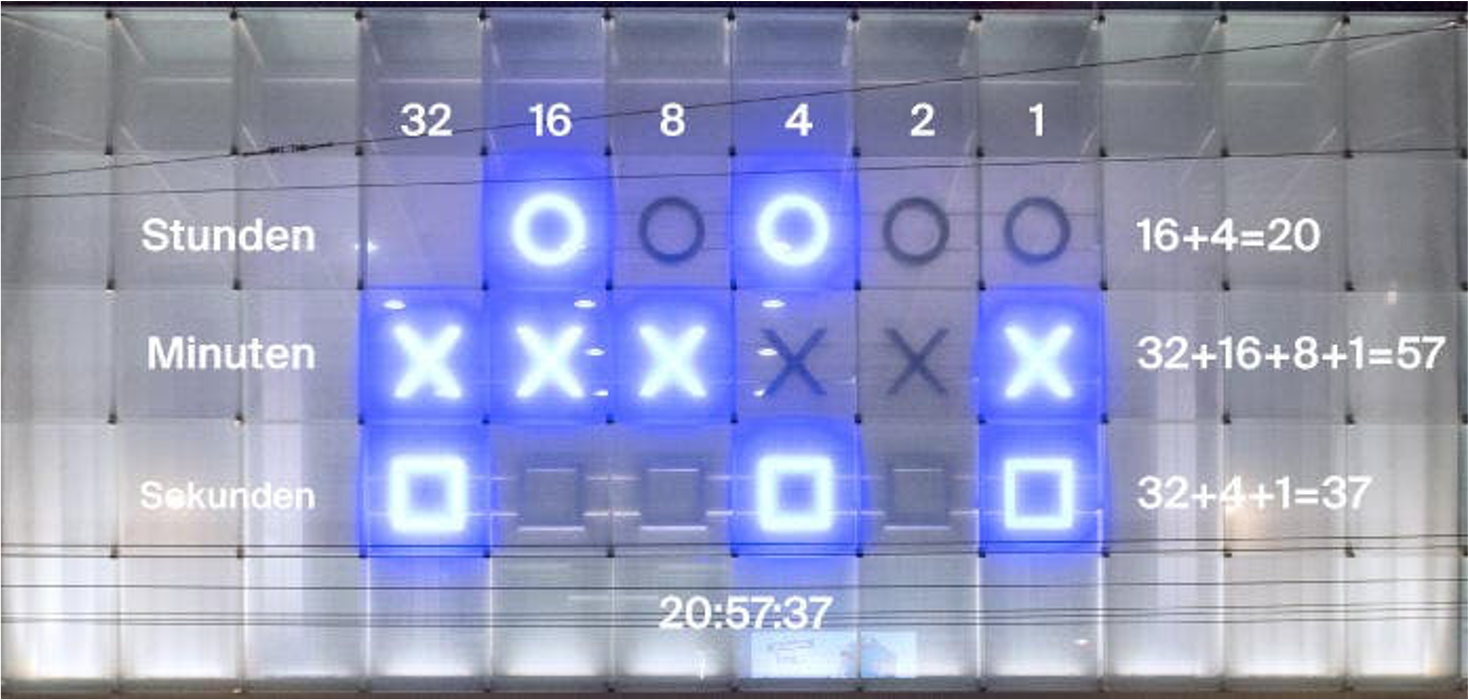
\includegraphics[width=0.9\textwidth]{binary_clock_read_help}
    \end{figure}
\end{frame}

\begin{frame}
    \frametitle{Warm-Up I}
    Uhrzeit 2:
    \begin{figure}[H]
        \centering
        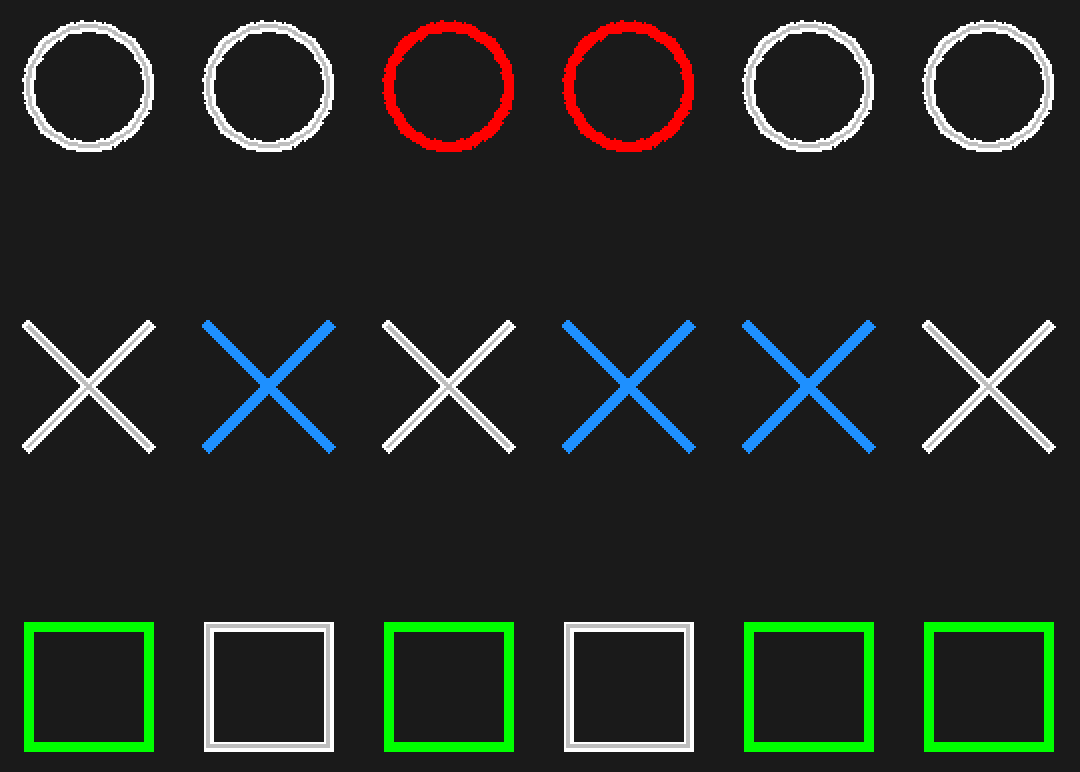
\includegraphics[width=0.7\textwidth]{12_22_43_dark}
    \end{figure}
    \onslide<2-> $$12:22:43$$
\end{frame}

\begin{frame}
    \frametitle{Warm-Up II}
    Frage: Wie weit kann man mit einer Hand zählen?
    \onslide<2->
    \begin{figure}[H]
        \centering
        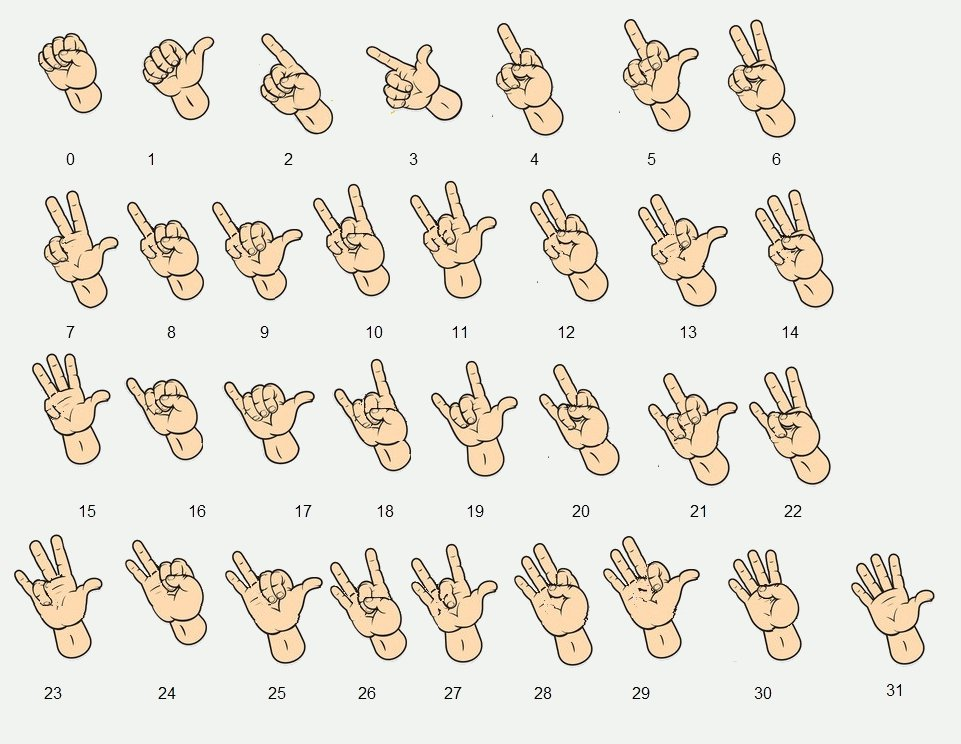
\includegraphics[width=0.7\textwidth]{binarycount}
    \end{figure}
\end{frame}

\begin{frame}
    \frametitle{Ziele}
    \begin{itemize}
        \item Wissen, was ein Zahlensystem ist
        \item \onslide<2-> Wissen, wie Dezimal \& Binärsystem aufgebaut sind
        \item \onslide<3-> Umrechnen Binärsystem $\rightarrow$ Dezimalsystem
        \item \onslide<4-> Code für Umrechnung schreiben
        % \item \onslide<4-> 
    \end{itemize}
\end{frame}

\begin{frame}
    \frametitle{Zahlensysteme}    
    \begin{definition}
        Ein \textbf{Zahlensystem} ist ein System, mit dem Zahlen dargestellt werden. Es wird durch seine \textbf{Basis} und seine \textbf{Nennwerte} festgelegt.
        \linebreak
        \linebreak
        Beispiele für Zahlensysteme sind das uns sehr vertraute Dezimalsystem, das Binärsystem (Basis $2$) oder das Hexadezimalsystem (Basis $16$).
    \end{definition}
\end{frame}

\begin{frame}
    \frametitle{Dezimalsystem}

    \begin{itemize}
        \item Das \textbf{Dezimalsystem} (auch \textbf{Zehnersystem}) ist das Zahlensystem mit \ldots
        \item \onslide<2-> Basis $10$ und \ldots
        \item \onslide<3-> Nennwerte $0,1,2,3,4,5,6,7,8,9$.
        \item \onslide<4-> Die Zahl $1903_{10}$ ist dann wie folgt zu interpretieren:
        \onslide<5->
        \begin{align*}
            \label{equ dezimalzahl in basis und nennwerten}
            \textcolor{blue}{1903}_{\textcolor{magenta}{10}}
            = \textcolor{blue}{1}\times \textcolor{magenta}{10}^{\textcolor{red}{3}} 
            + \textcolor{blue}{9}\times \textcolor{magenta}{10}^{\textcolor{red}{2}} 
            + \textcolor{blue}{0}\times \textcolor{magenta}{10}^{\textcolor{red}{1}} 
            + \textcolor{blue}{3}\times \textcolor{magenta}{10}^{\textcolor{red}{0}}
        \end{align*}
        \item \onslide<6-> Mit der \textit{kleinen Zahl unten rechts} ($\textcolor{magenta}{10}$) deuten wir an, dass die Zahl im Dezimalsystem zu betrachten ist. 
        \item \onslide<7-> Lässt man diese Zahl weg, schreibt man also z.B. $576$, so bedeutet dies (meistens), dass die Zahl im Dezimalsystem steht.
    \end{itemize}
\end{frame}

\begin{frame}
    \frametitle{Binärsystem}

    \begin{center}
        ``\textit{I told my friend 10 jokes about the binary system - He didn't get either of them!}''	
    \end{center}

    \onslide<2-> 

    \begin{definition}
        Die kleinste Informationseinheit ist das \textbf{Bit}, es hat zwei Möglichkeiten: es kann entweder $0$ oder $1$ sein.
        In der Welt der Elektrotechnik hat diese eine besondere Relevanz, da diese den beiden Zuständen `es fliesst kein Strom ($0$)' oder `es fliesst Strom ($1$)' entsprechen. 
        \onslide<3-> 
        \newline
        \newline
        Deshalb ist da das \textbf{Binärsystem} wichtig: Die Basis ist $2$ und die Nennwerte sind $0$ und $1$. Eine Binärzahl besteht also aus mehreren Bits.
    \end{definition}
\end{frame}

\begin{frame}
    \frametitle{Binärsystem}

    Das \textbf{Umrechnen einer Binärzahl in eine Dezimalzahl} geht ganz einfach. Für die Zahl $100101_2$ geht man wie folgt vor:
    \begin{align*}\begin{split}
        \textcolor{blue}{100101}_{\textcolor{magenta}{2}}
        &= \textcolor{blue}{1} \times \textcolor{magenta}{2}^{\textcolor{red}{5}}
        + \textcolor{blue}{0} \times \textcolor{magenta}{2}^{\textcolor{red}{4}}
        + \textcolor{blue}{0} \times \textcolor{magenta}{2}^{\textcolor{red}{3}}
        + \textcolor{blue}{1} \times \textcolor{magenta}{2}^{\textcolor{red}{2}}
        + \textcolor{blue}{0} \times \textcolor{magenta}{2}^{\textcolor{red}{1}}
        + \textcolor{blue}{1} \times \textcolor{magenta}{2}^{\textcolor{red}{0}}
        \\
        &= 32_{10} + 4_{10} + 1_{10}
        \\
        &= 37_{10}		
    \end{split}\end{align*}
\end{frame}

\begin{frame}
    \frametitle{Aufgaben lösen}
    Dossier auf OneNote (beinhaltet alle Theorie von heute)
    \begin{itemize}
        \item Aufgabe 2.1
        \item Aufgabe 3.1
        \item Aufgabe 3.2
        \item Aufgabe 3.3
        \begin{itemize}
            \vspace{-\topsep}
            \item Code: Binärzahl in Dezimalzahl
            \item alleine oder in 2er-Gruppe (keine 3er usw.)
            \item \textcolor{red}{Abgabe bis heute Abend per Teams}
            \item falls in Gruppe gearbeitet nur $1$ Abgabe
            \item keinen kopierten Code abgeben
        \end{itemize}
        
    \end{itemize}
\end{frame}

%%%%%%%%%%%%%%%%%%%%%%%%%%%%%%%%%%%%%%%%%%%%%%%%%%%%%%%%

\begin{frame}
    \LARGE
    Lektion 3: Dezimal- \& Binärsystem II
\end{frame}

\begin{frame}
    \frametitle{Warm-Up I}
    Welche Zahl (als Binär- und Dezimalzahl) wird hier dargestellt?
    \begin{figure}[H]
        \centering
        
\includegraphics[width=0.2\textwidth]{hand_5}
    \end{figure}
    \onslide<2-> $$101_2
    \onslide<3->= 2^2 + 2^0
    \onslide<4->= 4+1
    \onslide<5->= 5$$
\end{frame}

\begin{frame}
    \frametitle{Warm-Up I}
    Welche Zahl (als Binär- und Dezimalzahl) wird hier dargestellt?
    \begin{figure}[H]
        \centering
        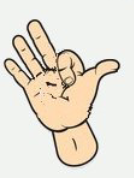
\includegraphics[width=0.2\textwidth]{hand_29}
    \end{figure}
    \onslide<2-> $$11101_2
    \onslide<3->= 2^4+2^3+2^2+2^0
    \onslide<4->= 16+8+4+1
    \onslide<5->= 29$$
\end{frame}

\begin{frame}
    \frametitle{Warm-Up I}
    Welche Zahl (als Binär- und Dezimalzahl) wird hier dargestellt?
    \begin{figure}[H]
        \centering
        
\includegraphics[width=0.2\textwidth]{hand_4}
        \hspace{-0.8cm}
        
\includegraphics[width=0.2\textwidth]{hand_4}
    \end{figure}
    \onslide<2-> $$00100\,00100_2
    \onslide<3->= 2^7+2^2
    \onslide<4->= 128 + 4
    \onslide<5->= 132$$
\end{frame}

\begin{frame}
    \frametitle{Warm-Up II}
    \begin{itemize}
        \setlength{\itemsep}{0pt}\setlength{\parskip}{0pt}
        \item \textbf{Wie weit kann man mit einer Hand zählen?}
        \item \onslide<2-> Antwort: 31
        \item \onslide<3->Warum?
        \item \onslide<4->Jeder Finger $2$ Möglichkeiten
        \item \onslide<5->5 Finger: $2\cdot2\cdot2\cdot2\cdot2 = 2^5 = 32$ Möglichkeiten
        \item \onslide<6->da Null eine Möglichkeit \ldots
        \item \onslide<7->höchste Zahl ist $2^5-1 = 32-1 = 31$
        \item \onslide<8->\textbf{Wie weit kann man mit zwei Händen zählen?}
        \item \onslide<9-> Antwort: $2^10-1 = 1023$
    \end{itemize}
    

\end{frame}

\begin{frame}
    \frametitle{Ziele}
    \begin{itemize}
        \item Dezimalzahlen in Binärzahlen umrechnen können
    \end{itemize}
\end{frame}

\begin{frame}
    \textbf{Plan}:
    \begin{enumerate}
        % \vspace{-\topsep}
        \onslide<2-> \item Umrechnung Dezimalzahl $\rightarrow$ Binärzahl deomonstrieren und erklären.\\
        ALTERNATIVE: Selbst studieren im Dossier.
        \onslide<3-> \item Tipps für A3.3, \textcolor{red}{fertig machen bis heute Abend und abgeben per Teams}
        \onslide<4-> \item HA korrigieren, Lösungen auf OneNote (ausser A3.3)
        \onslide<5-> \item restliche Aufgaben im Dossier: A3.4-3.6
    \end{enumerate}
\end{frame}

\begin{frame}
    \frametitle{Umrechnung: Dezimalzahl zu Binärzahl}
    $42_{10}$ als Binärzahl?
    \onslide<2-> $$\text{Schritt 1:} \quad 42                      \quad/\quad 2 \quad = \quad \onslide<3->\textcolor{blue}{21}    \quad \text{Rest:} \quad \textcolor{red}{0}$$  \vspace{-0.5cm}
    \onslide<4-> $$\text{Schritt 2:} \quad \textcolor{blue}{21}    \quad/\quad 2 \quad = \quad \onslide<5->\textcolor{magenta}{10} \quad \text{Rest:} \quad \textcolor{red}{1}$$  \vspace{-0.5cm}
    \onslide<6-> $$\text{Schritt 3:} \quad \textcolor{magenta}{10} \quad/\quad 2 \quad = \quad \onslide<7->\textcolor{green}{5}    \quad \text{Rest:} \quad \textcolor{red}{0}$$  \vspace{-0.5cm}
    \onslide<8-> $$\text{Schritt 4:} \quad \textcolor{green}{5}    \quad/\quad 2 \quad = \quad \onslide<9->\textcolor{orange}{2}   \quad \text{Rest:} \quad \textcolor{red}{1}$$  \vspace{-0.5cm}
    \onslide<10-> $$\text{Schritt 5:} \quad \textcolor{orange}{2}   \quad/\quad 2 \quad = \quad \onslide<11->\textcolor{cyan}{1}     \quad \text{Rest:} \quad \textcolor{red}{0}$$\vspace{-0.5cm}
    \onslide<12-> $$\text{Schritt 6:} \quad \textcolor{cyan}{1}     \quad/\quad 2 \quad = \quad \onslide<13->\textcolor{yellow}{0}   \quad \text{Rest:} \quad \textcolor{red}{1}$$
    \onslide<14->
    Das Resultat ist also:
    $\quad42_{10} = \textcolor{red}{101010}_2$
\end{frame}

\begin{frame}
    \frametitle{Umrechnung: Dezimalzahl zu Binärzahl}
    $37_{10}$ als Binärzahl? Kompakte Darstellung:
    \onslide<2->
    \begin{table}[H]
        \centering
        \renewcommand{\arraystretch}{1.5}
        \begin{tabular}{|c|c|}
        \hline
        \onslide<2->\textbf{37} & \\ \hline
        \onslide<3->18 &\onslide<4->  \textcolor{red}{1} \\ \hline
        \onslide<5->9  &\onslide<6->  \textcolor{red}{0} \\ \hline
        \onslide<7->4  &\onslide<8->  \textcolor{red}{1} \\ \hline
        \onslide<9->2  &\onslide<10-> \textcolor{red}{0} \\ \hline
        \onslide<11->1 &\onslide<12-> \textcolor{red}{0} \\ \hline
        \onslide<13->0 &\onslide<14-> \textcolor{red}{1} \\ \hline
    \end{tabular}
    \end{table}
    \onslide<15->
    Das Resultat ist also
    $$37_{10} = \textcolor{red}{100101}_2$$
\end{frame}

%%%%%%%%%%%%%%%%%%%%%%%%%%%%%%%%%%%%%%%%%%%%%%%%%%%%%%%%

\begin{frame}
    \LARGE
    Lektion 4: Rechnen im Binärsystem
\end{frame}

\begin{frame}
    \frametitle{Ziele}
    \begin{itemize}
        \item Binärzahlen schriftlich addieren können
    \end{itemize}
\end{frame}

\begin{frame}
    \frametitle{Warm-Up I: Binärzahl $\rightarrow$ Dezimalzahl}

    \begin{itemize}
        \item \textbf{Umwandlung Binärzahl $\rightarrow$ Dezimalzahl}
        \item \onslide<2-> Binäruhr lesen (TigerJython Programm)
    \end{itemize}
\end{frame}

\begin{frame}
    \frametitle{Warm-Up II: Dezimalzahl $\rightarrow$ Binärzahl}
    
    \begin{itemize}
        \item \textbf{Umwandlung Dezimalzahl $\rightarrow$ Binärzahl}
        \item \onslide<2-> Restwertalgorithmus
    \end{itemize}
\end{frame}


\begin{frame}
    \frametitle{Warm-Up II: Dezimalzahl $\rightarrow$ Binärzahl}
    $37_{10}$ als Binärzahl? Restwertalgorithmus:
    \onslide<2->
    \begin{table}[H]
        \centering
        \renewcommand{\arraystretch}{1.5}
        \begin{tabular}{|c|c|}
        \hline
        \onslide<2->\textbf{37} & \\ \hline
        \onslide<3->18 &\onslide<4->  \textcolor{red}{1} \\ \hline
        \onslide<5->9  &\onslide<6->  \textcolor{red}{0} \\ \hline
        \onslide<7->4  &\onslide<8->  \textcolor{red}{1} \\ \hline
        \onslide<9->2  &\onslide<10-> \textcolor{red}{0} \\ \hline
        \onslide<11->1 &\onslide<12-> \textcolor{red}{0} \\ \hline
        \onslide<13->0 &\onslide<14-> \textcolor{red}{1} \\ \hline
    \end{tabular}
    \end{table}
    \onslide<15->
    Das Resultat ist also
    $$37_{10} = \textcolor{red}{100101}_2$$
\end{frame}

\begin{frame}
    \frametitle{Warm-Up II: Dezimalzahl $\rightarrow$ Binärzahl}
    
    Wende nun selbst Restwertalgorithmus an um folgende Dezimalzahlen in Binärzahlen umzuwandeln:
    \begin{enumerate}
        \item $29_{10}  = \,?_2$ % 11101
        \item $43_{10}  = \,?_2$ % 10 1011
        \item $64_{10}  = \,?_2$ % 100 0000
        \item $100_{10} = \,?_2$ % 110 0100
    \end{enumerate}
    \onslide<2->Lösungen:
    \begin{enumerate}
        \item $29_{10}  =   1\,1101_2$
        \item $43_{10}  =  10\,1011_2$
        \item $64_{10}  = 100\,0000_2$
        \item $100_{10} = 110\,0100_2$
    \end{enumerate}
\end{frame}


\begin{frame}
    \frametitle{Auftrag: Addition von Binärzahlen}

    \begin{itemize}
        \item Dossier II
        \item \onslide<2->Löse Aufgabe in Kapitel 3.1:
        \item \onslide<3->Aufgabe 3.7: Schriftliches Addieren von Dezimalzahlen und Binärzahlen
        \item \onslide<4->Aufgabe 3.8: Code schreiben, der Binärzahlen addiert
    \end{itemize}
\end{frame}


% \begin{frame}
%     \frametitle{}
%     \begin{itemize}
%         \item 
%         \item \onslide<2-> 
%         \item \onslide<3-> 
%         \item \onslide<4-> 
%     \end{itemize}
% \end{frame}

\end{document}
